\documentclass{acm_proc_article-sp}

\begin{document}

\title{Supervised Learning}
\subtitle{Writeup for Assignment 01 - CS 6741}

\author{
\alignauthor
Magahet Mendiola
}
\date{}

\maketitle
\begin{abstract}
An analysis of two machine learning classification problems, including an evaluation of various learning algorithms and an exploration into the 
\end{abstract}
 

%a description of your classification problems, and why you feel that they are interesting. Think hard about this. To be at all interesting the problems should be non-trivial on the one hand, but capable of admitting comparisons and analysis of the various algorithms on the other.

\section{Classification Problems}

Two classification datasets have been chosen based on the following criteria. First, each dataset was required to include a minimum of 3,000 sample instances to insure that sufficient data was available to evaluate each learning algorithm. A standardized test set was created by taking a uniformally random sample

\section{Classification 1 - Poison Mushrooms}

The first dataset we shall examine is titled, Mushroom \cite{Bache+Lichman:2013} and was chosen from the UCI ML Repository. The classification task for this dataset is to determine whether a given mushroom is edible or poisonous based on the specimen's physical attributes. There are 22 attributes which describe the physical appearance and olfactory perception of each sample. A full description of attributes can be found at http://archive.ics.uci.edu/ml/datasets/Adult.


\section{Classification 2 - xxxx}

Our second dataset was also chosen from the UCI ML Repository and is titled, Adult \cite{Bache+Lichman:2013}. The classification task in this case is to determine if one's household income exeeds \$50,000/yr based on 14 biographical attributes. The data was collected from a census database from 1994. Attributes include the subject's age, level of education, marital-status, occupation, race, sex, etc. The full description of attributes can be found at http://archive.ics.uci.edu/ml/datasets/Adult.



\section{Algorithm Evaluations}
%the training and testing error rates you obtained running the various learning algorithms on your problems. At the very least you should include graphs that show performance on both training and test data as a function of training size (note that this implies that you need to design a classification problem that has more than a trivial amount of data) and--for the algorithms that are iterative--training times.

\subsection{Learning Curve}

\begin{figure}[te-c45]
\centering
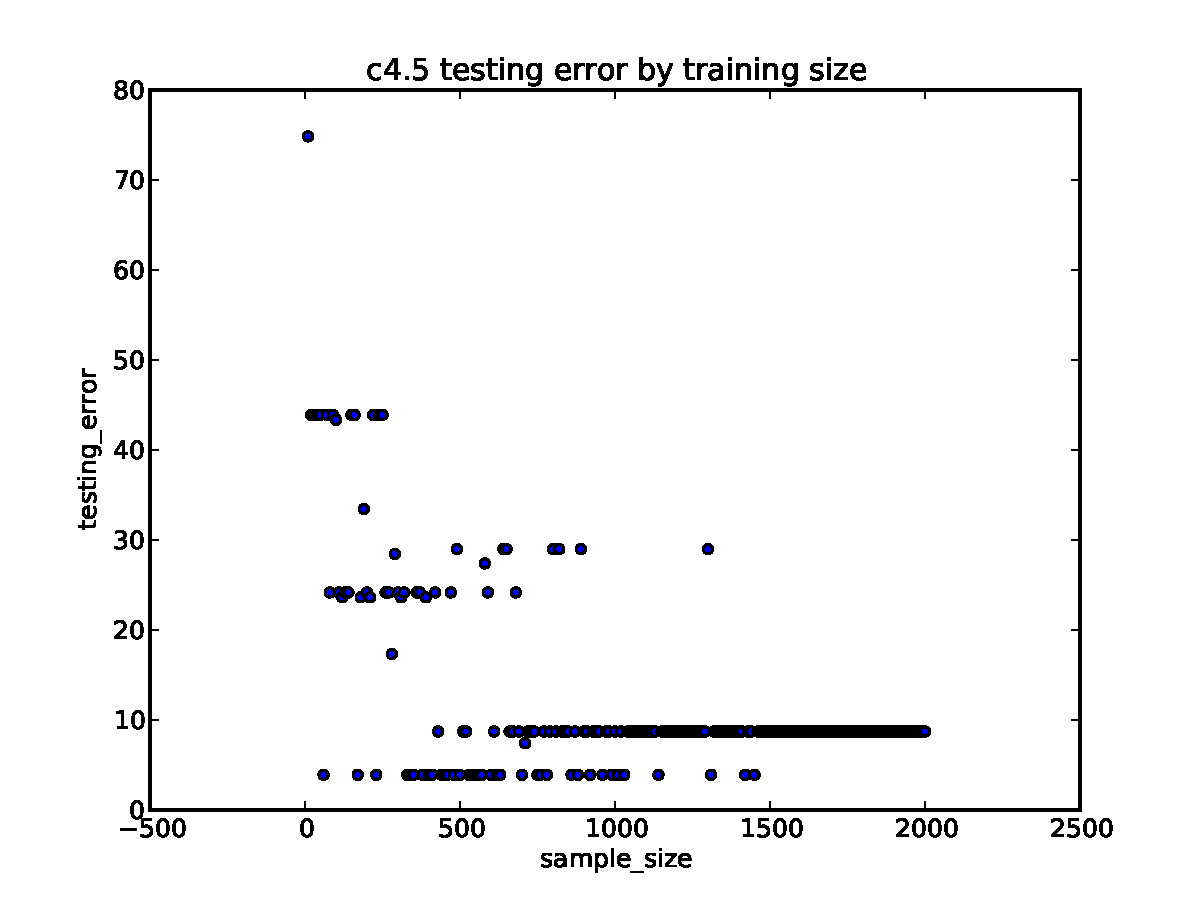
\includegraphics[width=3in]{data/agaricus-lepiota/learning-curve-10to2000/test-error-c45.pdf}
\caption{Test Error by Training Size - C4.5}
\end{figure} 

\begin{figure}[te-perceptron]
\centering
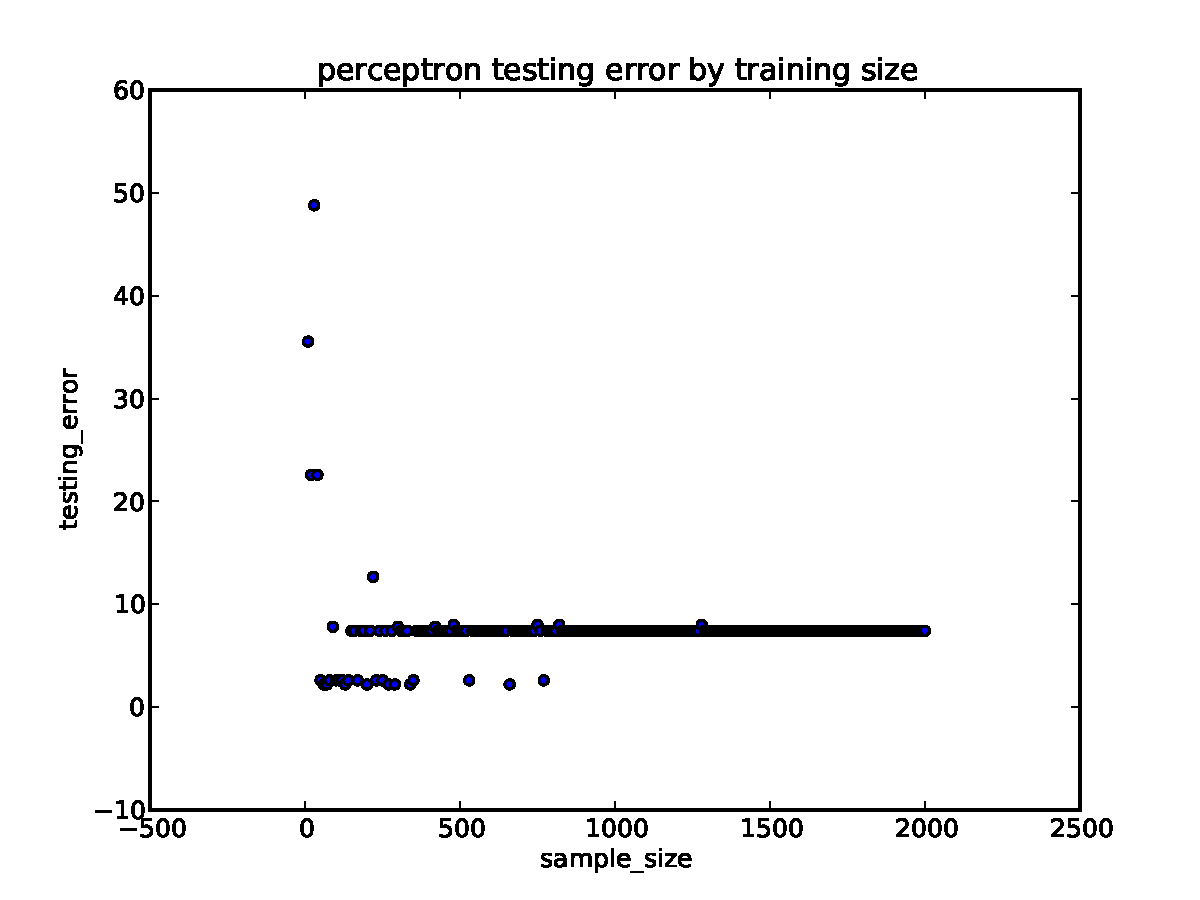
\includegraphics[width=3in]{data/agaricus-lepiota/learning-curve-10to2000/test-error-perceptron.pdf}
\caption{Test Error by Training Size - ANN}
\end{figure} 

%\begin{figure}[]
%\centering
%\includegraphics[width=3in]{data/agaricus-lepiota/learning-curve-10to2000/test-error-.pdf}
%\caption{Test Error by Training Size - }
%\end{figure} 

%\begin{figure}[]
%\centering
%\includegraphics[width=3in]{data/agaricus-lepiota/learning-curve-10to2000/test-error-.pdf}
%\caption{Test Error by Training Size - }
%\end{figure} 

%\begin{figure}[]
%\centering
%\includegraphics[width=3in]{data/learning-curve-10to2000/test-error-.pdf}
%\caption{Test Error by Training Size - }
%\end{figure} 


\subsection{Decision Trees}
%Decision Trees. For the decision tree, you should implement or steal a decision tree algorithm. Be sure to use some form of pruning. You are not required to use information gain (for example, there is something called the GINI index that is sometimes used) to split attributes, but you should describe whatever it is that you do use.

\subsection{Neural networks}
%For the neural network you should implement or steal your favorite kind of network and training algorithm. You may use networks of nodes with as many layers as you like and any activation function you see fit.

\subsection{Boosting}
%Implement a boosted version of your decision trees. As before, you will want to use some form of pruning, but presumably because you're using boosting you can afford to be much more aggressive about your pruning.

\subsection{Support Vector Machines}
%You should implement (for sufficently loose definitions of implement including download) SVMs. This should be done in such a way that you can swap out kernel functions. I'd like to see at least two.

\subsection{k-nearest neighbor}
%You should implement kNN. Use different values of k.


\section{Analysis}

\subsection{Overview of Results}
%analyses of your results. Why did you get the results you did?

\subsection{Algorithm Comparison}
%Compare and contrast the different algorithms. What sort of changes might you make to each of those algorithms to improve performance? How fast were they in terms of wall clock time? Iterations? Would cross validation help (and if it would, why didn't you implement it?)? How much performance was due to the problems you chose? How about the values you chose for learning rates, stopping criteria, pruning methods, and so forth (and why doesn't your analysis show results for the different values you chose?)? Which algorithm performed best? How do you define best? Be creative and think of as many questions you can, and as many answers as you can.



\bibliographystyle{abbrv}
\bibliography{term-paper}
\begin{thebibliography}{10}

\bibitem{Bache+Lichman:2013}
K. Bache and M. Lichman
\newblock UCI Machine Learning Repository
\newblock 2013
\newblock http://archive.ics.uci.edu/ml
\newblock University of California, Irvine, School of Information and Computer Sciences

%\bibitem{Zhong:Osteo}
%L.~Zhong, D.~El-Daye, B.~Kaufman, N.~Tobaoda, T.~Mohamed, and M.~Liebschner.
%\newblock Osteoconduct: Wireless body-area communication based on bone
  %conduction.
%\newblock In {\em in Proc. Int. Conf. Body Area Networks (BodyNets)}, June
  %2007.

\end{thebibliography}
\end{document}
